\documentclass[11pt,a4paper]{article}
\usepackage[margin=1in]{geometry}
\usepackage{graphicx}
\usepackage{booktabs}
\usepackage{amsmath}
\usepackage{hyperref}
\usepackage{float}

\title{\textbf{Passive Thermal Design of a 6U Small Satellite Under a High-Beta Bounding Hot Case}}
\author{\textbf{Lead Thermal Engineer} \\ \textit{Aerospace Systems Engineering Division}}
\date{}

\begin{document}

\maketitle

\begin{abstract}
This report documents the preliminary passive thermal design and radiator sizing trade-off analysis of a high-power 6U technology-demonstration CubeSat in a circular 600 km dawn-dusk Sun-Synchronous Orbit (SSO). In dawn-dusk SSO configurations, high solar beta angles during solstices drive near-continuous solar exposure, presenting extreme over-temperature challenges for internal avionics and battery packs. We present \textbf{Passive Redesign v2}, which eliminates the need for active cooling or deployable mechanisms. The redesign uses passive thermal zoning, surface coating selection (AZ-93 silicate paint and silvered FEP tape), and orbit-attitude-dependent radiator placement on the anti-Sun cross-track face. A dual-axis system-level radiator sizing sweep reveals that a $0.02\text{ m}^2$ radiator offers the optimal balance between hot-case thermal safety margin (avionics peak at $39.2^\circ$C) and cold-case heater power penalties ($5.92$ Wh/orbit).
\end{abstract}

\section{Introduction}
Modern small satellites are increasingly packed with high-power payloads and avionics, leading to significant internal power dissipation. A standard 6U CubeSat ($10\text{ cm} \times 20\text{ cm} \times 30\text{ cm}$) technology-demonstrator requires robust thermal architecture to operate under bounding orbital conditions. 

This study focuses on a 6U spacecraft in a circular 600 km dawn-dusk SSO with an inclination of $\approx 97.8^\circ$. Under solstice conditions, the orbit plane tilts relative to the sun vector, yielding a high beta angle ($\beta = 74^\circ$) that exceeds the critical shadow angle ($\approx 66.07^\circ$), causing the satellite to remain in continuous sunlight. The SSO geometry and sunlit schedule are shown in Figure 1.

\begin{figure}[H]
\centering
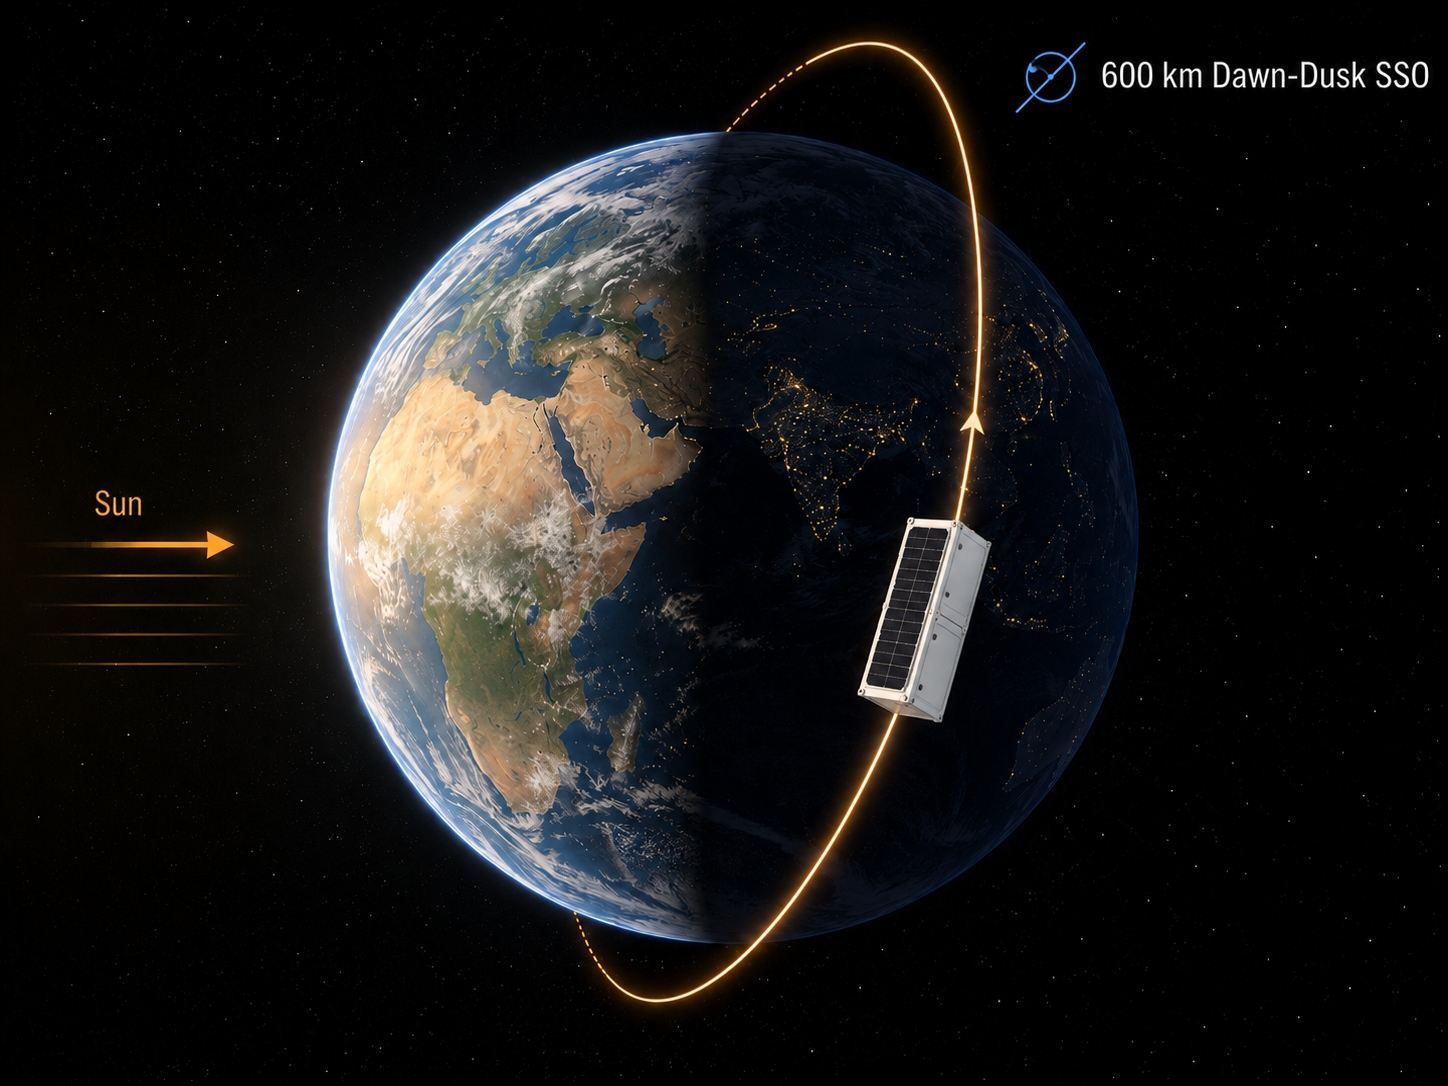
\includegraphics[width=0.75\textwidth]{sso_orbit.png}
\caption{Circular 600 km Dawn-Dusk SSO Orbit Geometry, illustrating the permanent solar illumination vector on the cross-track panel.}
\end{figure}

\section{Thermal Limits and Component Specifications}
Thermal node mass, capacitance, and operational limits are traceable to engineering standards. The component details are listed in Table 1.

\begin{table}[H]
\centering
\caption{Component Mass, Capacitance, and Temperature Limits}
\vspace{0.2cm}
\resizebox{\textwidth}{!}{%
\begin{tabular}{lccccc}
\toprule
\textbf{Node ID} & \textbf{Mass [kg]} & \textbf{$c_p$ [J/kg$\cdot$K]} & \textbf{Min Limit [$^\circ$C]} & \textbf{Max Limit [$^\circ$C]} & \textbf{Internal Diss. [W]} \\
\midrule
Battery & 1.5 & 800.0 & -10.0 & 45.0 & 0.5 \\
Avionics & 1.0 & 900.0 & -20.0 & 60.0 & 10.0 -- 15.0 \\
Payload & 2.0 & 900.0 & -10.0 & 50.0 & 0.0 -- 15.0 \\
Structure & 3.0 & 900.0 & -40.0 & 80.0 & 0.0 \\
Radiator & 0.5 & 900.0 & -100.0 & 100.0 & 0.0 \\
External Shell & 1.5 & 900.0 & -100.0 & 100.0 & 0.0 \\
\bottomrule
\end{tabular}%
}
\end{table}

The 6-node lumped-parameter thermal network architecture, conductive couplings $G_{ij}$, and external load interfaces are shown schematically in Figure 2.

\begin{figure}[H]
\centering
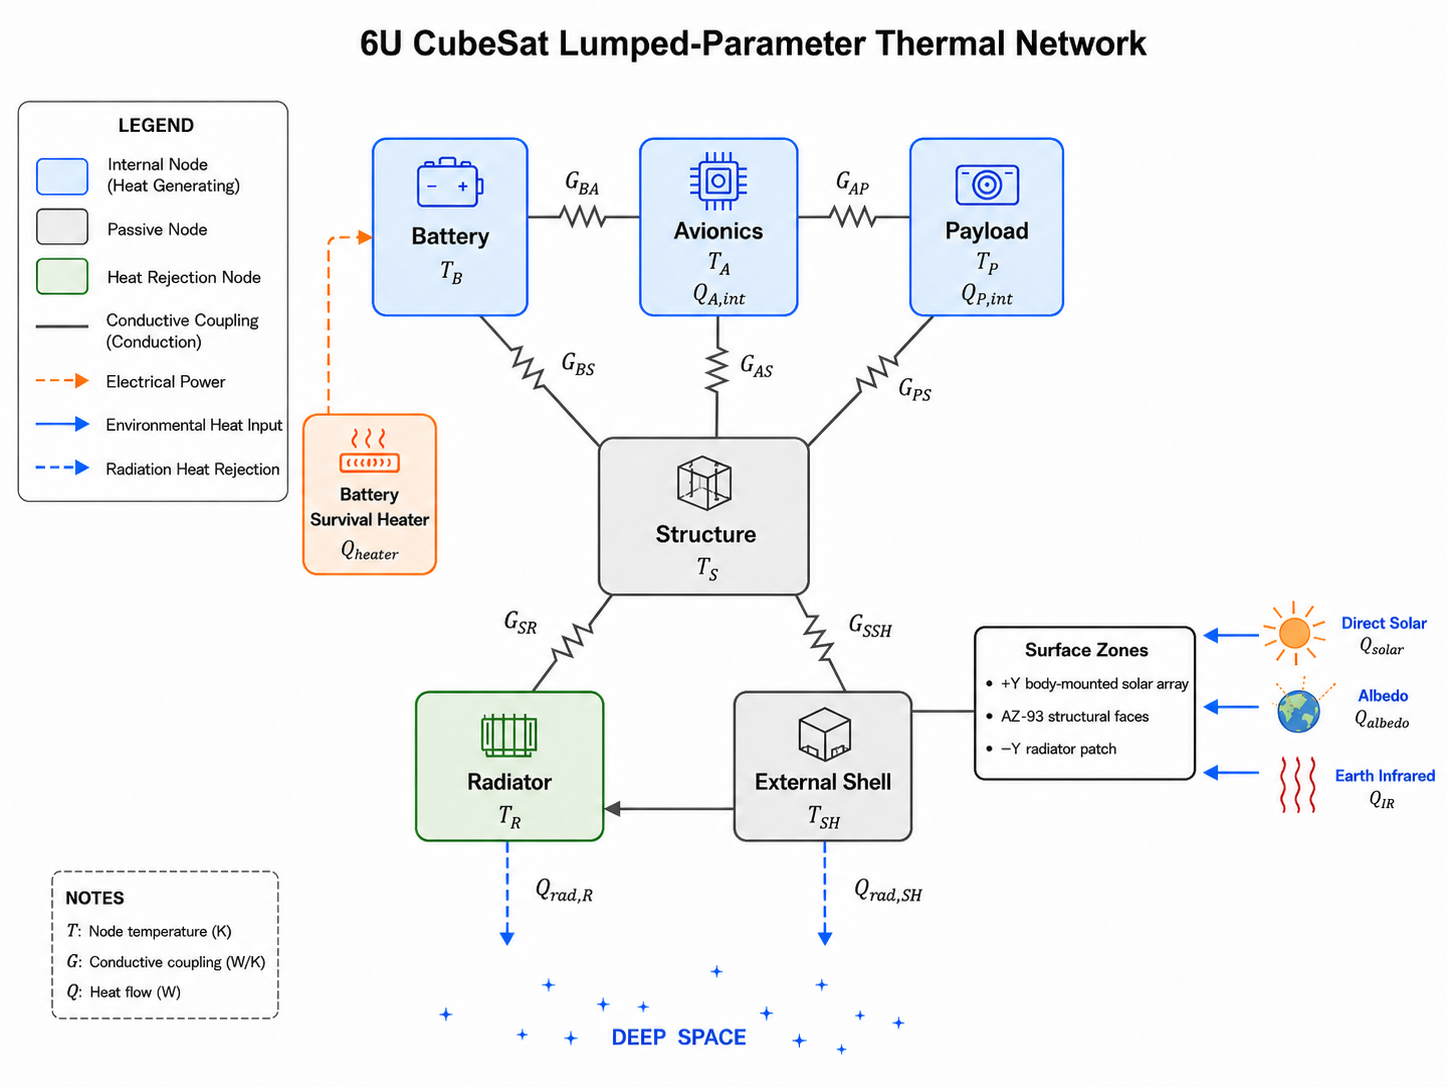
\includegraphics[width=0.75\textwidth]{thermal_network.png}
\caption{6-Node Lumped Parameter Thermal Network diagram, showing inter-node conductive paths and environmental radiation links.}
\end{figure}

\section{Material Library and Optical Properties}
All thermo-optical coatings used in this design are canonical candidates sourced directly from the \href{https://www.nasa.gov/smallsat-institute/sst-soa/thermal-control/}{NASA SmallSat State of the Art (SoA) Thermal Control} webpage, specifically Tables 7-3 and 7-4. The material properties catalog is summarized in Table 2.

\begin{table}[H]
\centering
\caption{Material Library and BOL Optical Properties}
\vspace{0.2cm}
\resizebox{\textwidth}{!}{%
\begin{tabular}{llcccl}
\toprule
\textbf{Material ID} & \textbf{Intended Role} & \textbf{$\alpha_s$ (BOL)} & \textbf{$\epsilon_{IR}$} & \textbf{NASA Source} & \textbf{Concise Description} \\
\midrule
AZ-93 Silicate & External shell & 0.16 & 0.90 & Table 7-3 & Inorganic white thermal paint \\
0.005$''$ FEP/Ag/Inconel & Primary radiator & 0.07 & 0.79 & Table 7-4 & Second-surface silvered FEP tape \\
VDA/200HN/PSA & Reference insulation & 0.08 & 0.03 & Table 7-4 & Metallized tape, very low emissivity \\
Z306 Polyurethane & Comparison paint & 0.92 & 0.89 & Table 7-3 & Matte black polyurethane paint \\
solar\_cell\_assembly & Solar panels & 0.73 & 0.82 & Section 7.1 & Body-mounted solar cells \\
\bottomrule
\end{tabular}%
}
\end{table}

\section{Baseline Failure Analysis}
The initial baseline configuration mapped high-absorptance black paint ($\alpha = 0.92, \epsilon = 0.89$) to several outer shell faces representing solar panel substrates. Under the bounding hot case ($\beta = 74^\circ$), the large surface absorption caused extreme solar heat loading. This resulted in catastrophic thermal limits breach across multiple nodes (Battery peaking at $80.6^\circ$C, Avionics peaking at $81.6^\circ$C). 

Additionally, using a low-emissivity material (like metallized VDA tape, $\epsilon = 0.03$) as a radiator was shown to cause thermal traps, raising avionics to $104.1^\circ$C due to the inability to reject heat to deep space.

\section{Passive Redesign v2 Architecture}
To resolve these violations passively, we implemented three key solutions in Redesign v2:
\begin{itemize}
    \item \textbf{Thermal Surface Zoning}: We mapped AZ-93 white paint ($\alpha = 0.16, \epsilon = 0.90$) to five non-power shell faces to minimize solar absorption while maximizing deep-space emittance.
    \item \textbf{Radiator Face Orientation Physics}: In dawn-dusk SSO, the cross-track $+Y$ face is permanently Sun-facing, while the opposite $-Y$ face is permanently shaded (anti-Sun). The dedicated radiator ($0.02\text{ m}^2$ silver FEP tape, $\alpha=0.07, \epsilon=0.79$) was relocated to the anti-Sun $-Y$ face to achieve the lowest integrated environmental heat load.
    \item \textbf{Solar Cell Electrical Offset}: Since $18\%$ of the absorbed solar energy on the solar arrays is converted to electricity and exported out of the thermal network, we applied an electrical conversion offset:
    \begin{equation}
        \alpha_{\text{eff}} = \alpha_s - \eta_{\text{elec}} = 0.73 - 0.18 = 0.55
    \end{equation}
\end{itemize}

Figure 3 illustrates the surface coating allocations and zoning layout for the redesigned spacecraft.

\begin{figure}[H]
\centering
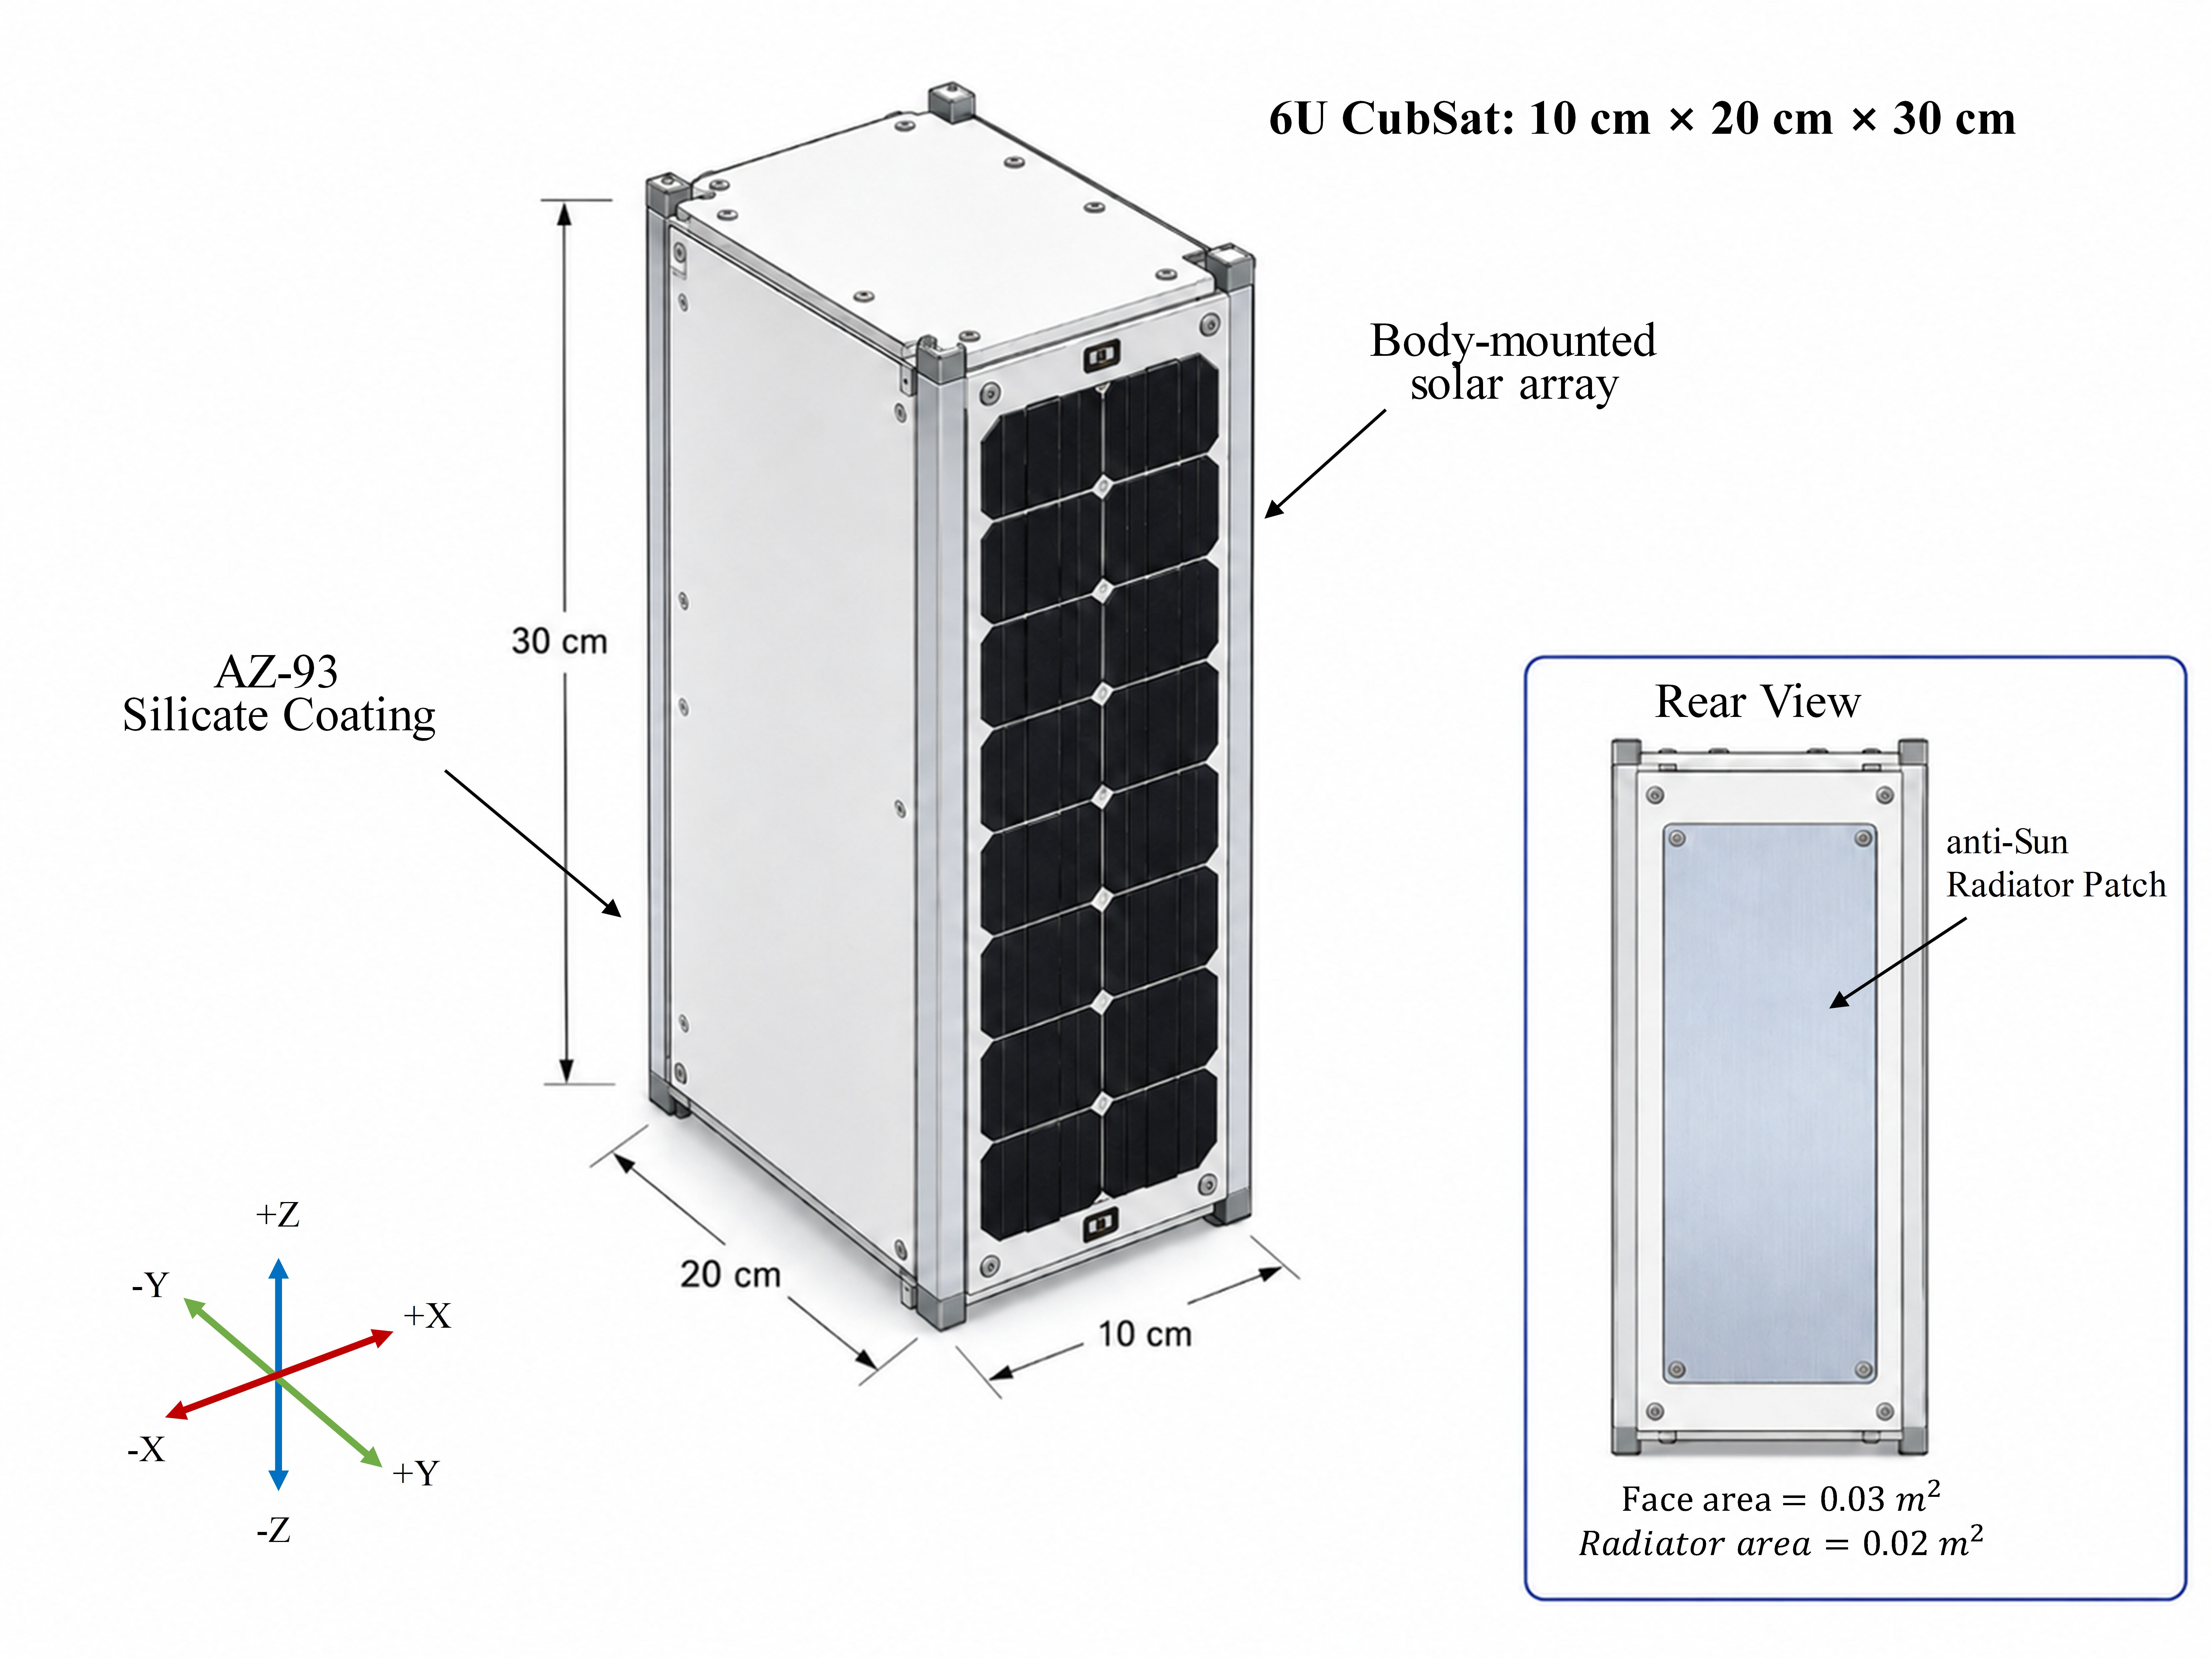
\includegraphics[width=0.65\textwidth]{thermal_zoning.png}
\caption{Spacecraft Passive Thermal Zoning layout (Redesign v2), showing body-mounted solar cell arrays on the Sun-facing $+Y$ face, AZ-93 white paint on the general shell, and the silver FEP radiator on the anti-Sun $-Y$ face.}
\end{figure}

\section{Simulation Results}
Applying the Redesign v2 architecture, all scenarios successfully converged to PASS conditions. Table 3 summarizes the steady-state node temperatures.

\begin{table}[H]
\centering
\caption{Steady-State Temperature Ranges under Redesign v2}
\vspace{0.2cm}
\resizebox{\textwidth}{!}{%
\begin{tabular}{lccc}
\toprule
\textbf{Node ID} & \textbf{Nominal ($\beta = 65^\circ$) [$^\circ$C]} & \textbf{Bounding Hot ($\beta = 74^\circ$) [$^\circ$C]} & \textbf{Cold Case ($\beta = 60^\circ$) [$^\circ$C]} \\
\midrule
Battery & 14.8 to 15.1 & 35.0 to 35.4 & 5.0 to 10.0 \\
Avionics & 16.4 to 17.1 & 38.1 to 39.2 & -0.8 to 0.8 \\
Payload & 14.1 to 17.7 & 34.0 to 40.3 & -1.7 to -0.5 \\
Structure & 13.2 to 14.2 & 33.5 to 34.8 & -2.2 to -0.1 \\
Heater Duty & 0.0\% & 0.0\% & 36.7\% \\
Heater Energy & 0.0 Wh & 0.0 Wh & 5.92 Wh/orbit \\
\bottomrule
\end{tabular}%
}
\end{table}

\section{Radiator Sizing System-Level Trade-Off}
A sweep of radiator area $A_{\text{rad}}$ from $0.02$ to $0.06\text{ m}^2$ was performed across all three scenarios to evaluate the trade-off between hot-case avionics peak temperature and cold-case heater power draw (Table 4).

\begin{table}[H]
\centering
\caption{Radiator Area Sweep Trade-Off Results}
\vspace{0.2cm}
\resizebox{\textwidth}{!}{%
\begin{tabular}{ccccc}
\toprule
\textbf{Area [$m^2$]} & \textbf{Hot Peak Avionics [$^\circ$C]} & \textbf{Cold Min Battery [$^\circ$C]} & \textbf{Cold Heater Duty [\%]} & \textbf{Cold Heater Energy [Wh]} \\
\midrule
0.02 & 39.17 & 5.00 & 36.7\% & 5.92 \\
0.03 & 34.87 & 5.00 & 41.5\% & 6.69 \\
0.04 & 31.15 & 5.00 & 49.0\% & 7.90 \\
0.05 & 27.80 & 5.00 & 63.6\% & 10.26 \\
0.06 & 24.81 & 4.99 & 60.9\% & 9.81 \\
\bottomrule
\end{tabular}%
}
\end{table}

Increasing the radiator size significantly drops the hot-case peak temperature, but imposes a severe $73\%$ heater energy penalty in the cold case. Due to strict power limitations on small satellites, the **$0.02\text{ m}^2$ radiator size is selected as the optimum thermal design**.

\section{Visualizations and Design Analysis}
The transient temperature response and parameter sizing trade-offs are visualized below. Figure 4 illustrates the nodal temperature histories under the continuous sunlight bounding hot case, showing stable convergence. Figure 5 depicts the dual-axis trade-off between peak hot avionics temperatures and cold battery margins across various radiator areas.

\begin{figure}[H]
\centering
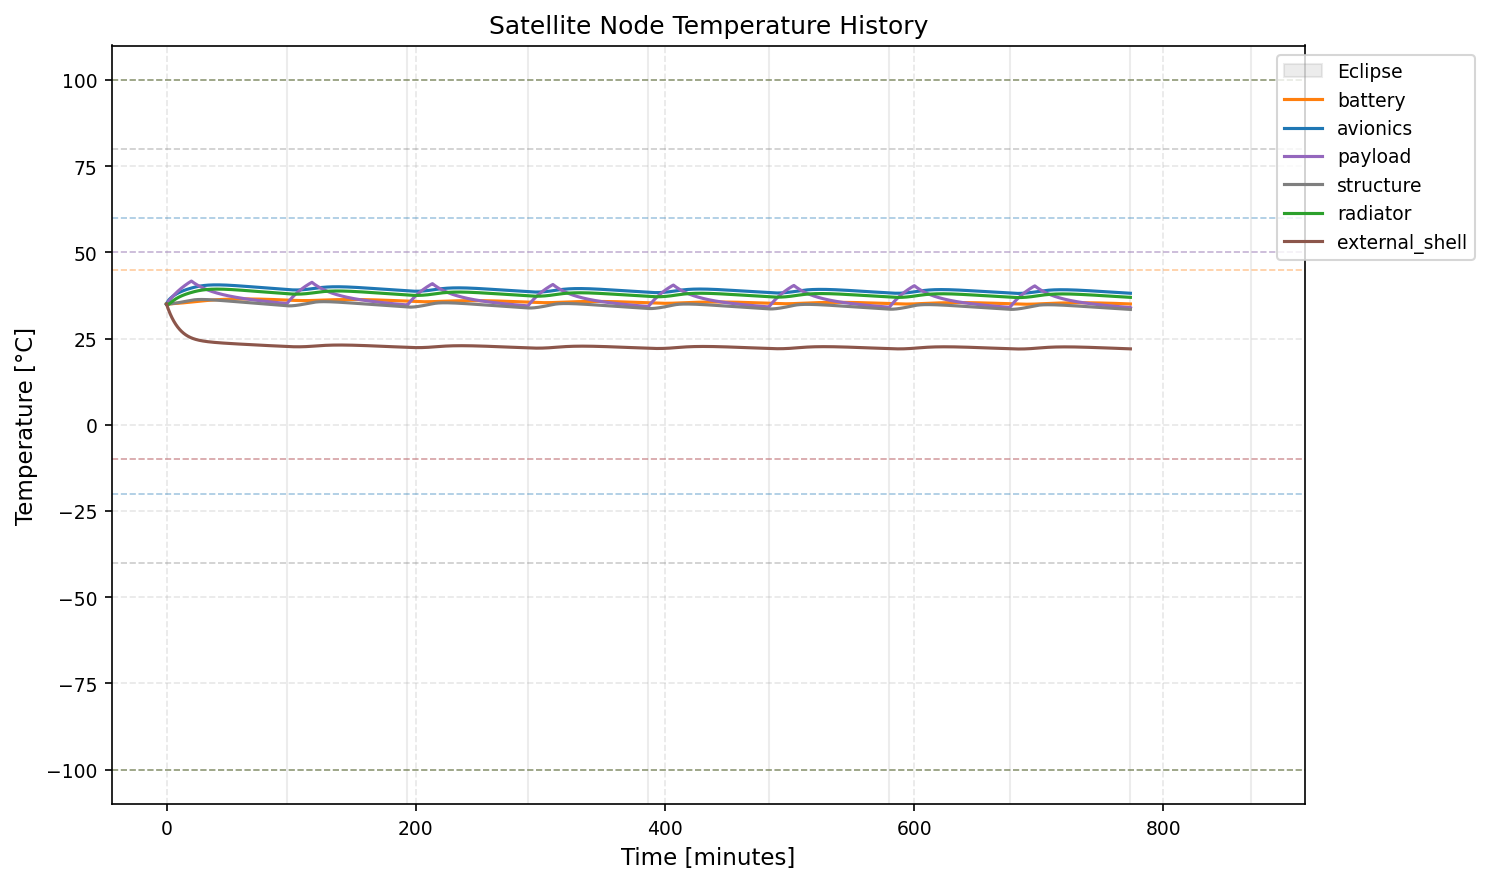
\includegraphics[width=0.7\textwidth]{../outputs/bounding_hot/temperature_history.png}
\caption{Nodal Temperature Histories Under Bounding Hot Case ($\beta = 74^\circ$, Continuous Sunlight Dawn-Dusk SSO Solstice).}
\end{figure}

\begin{figure}[H]
\centering
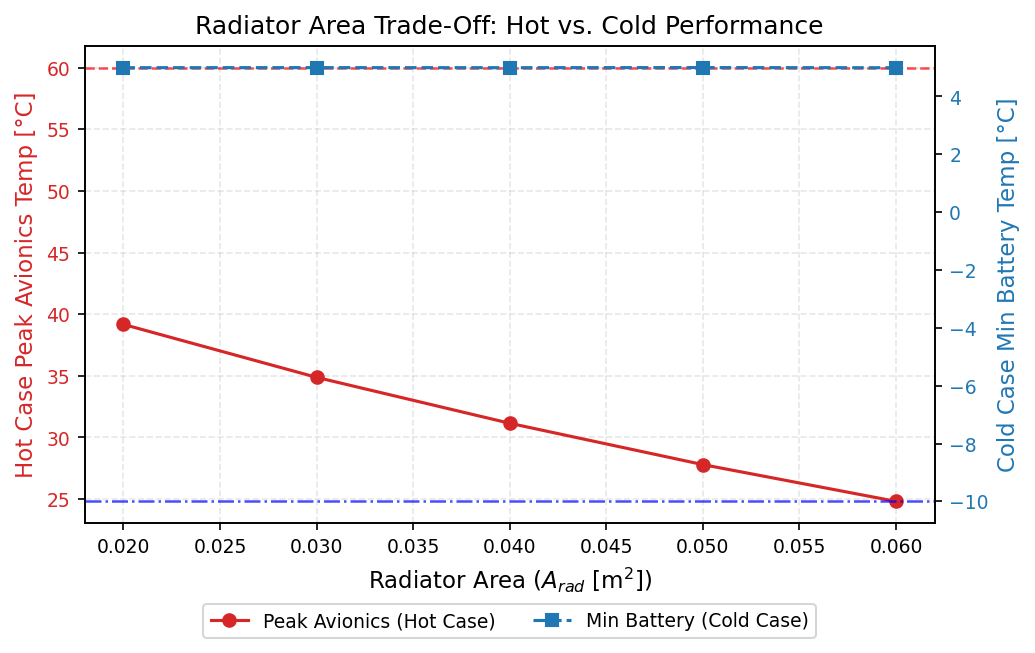
\includegraphics[width=0.7\textwidth]{../outputs/trades/radiator_area_system_trade.png}
\caption{Dual-Axis Radiator Sizing Trade-Off (Hot Case Peak Avionics Temp vs. Cold Case Min Battery Temp).}
\end{figure}

\section{Conclusion}
This report demonstrates that a rigorous passive thermal redesign utilizing surface zoning, anti-Sun radiator placement, and electrical power offset calculations successfully resolves the hot-case over-temperature limits of a 6U CubeSat in 600 km dawn-dusk SSO. Sizing trades highlight the importance of balancing radiator design to minimize cold-case heater power penalties.

\end{document}
